\chapter{Elektronik}
\renewcommand{\kapitelautor}{Autor: Lucas Ullrich}

%%%%%%%%%%%%%%%%%%%%%%%%%%%%%%%%%%%%%%%%%%%%%%%%%%%%%%%%%%%%%%%%%%%%%%%%%%%%%%%
\section{Allgemeine technische Planung}
Für die Umsetzung eines autonomen Fluges sind diverse Sensoren sowie eine entsprechende Auswertung der gelieferten Daten notwendig.
Alle Daten müssen an einem zentralen Ort für eine Auswertung zusammenlaufen, aus diesen können schließlich die notwendigen Flugparameter ermittelt werden.

  \subsection{Benötigte Elemente}
  Eine eigens entwickelte Ansteuerung der einzelnen Rotoren gestaltet sich als sehr umfangreich, deshalb wird ein fertiger Flight-Controller verwendet.
  Das System selbst basiert auf einer Modulbauweise, so könenn einzelne Komponenten, je nach Bedarf, includiert oder excludiert werden.
  Sämtliche Informationen werden über einen PIC-Mikrocontroller geleitet und über diesen ausgewertet.

    \subsubsection{PIC}
    Als zentrale Recheneinheit wird ein PIC18F46K22 verwendet. Dieser bietet ausreichend viel Speicherplatz und Pins für eine Testphase und kann mit einer Geschwindigkeit
    von bis zu $\SI{64}{\mega\hertz}$ intern getaktet werden. So ist keine aufwändige Oszillator-Schaltung notwendig und es ist eine vernünftig hohe Geschwindigkeit bei der
    Auswertung erzielbar.

    Der PIC ist dabei für die Auswertung der Kamera, des Ultraschallsensors, des Fernsteuerungsempfängers AR610 von Spektrum sowie dem WLAN-Modul zuständig.
    Je nach gewähltem Flugmodus steurt der PIC einen Multiplexer so an, dass ein autonomer oder manueller Flug möglich ist.
    Außerdem werdn von ihm die Servor-Impulse für den Flightcontroller ausgegeben.

    \subsubsection{DJI NAZA-M lite, Flamewheel F550}
    Der Flightcontroller NAZA-M lite von DJI ist ein bereits mit dem Flamewheel F550 ARF-Kit (Almost Ready to Fly) verkaufter Flugregler.
    Er ist dafür zuständig, dass die ankommenden Steuerimpulse namens Aileron, Elevator, Throttle und Rudder richtig verarbeitet werden.
    Dabei findet bereits eine automatische Regelung der Fluglage statt, der Hexacopter neigt sich also nicht über einen bestimmten Winkel von \textcolor{red}{$\SI{1234567}{\degree}$}.
    Ebenso werden die einzelnen Rotoren bereits so angesteuert, dass hier kein externer Eingriff mehr notwendig ist.
    \begin{figure}[H]
      \begin{centering}
        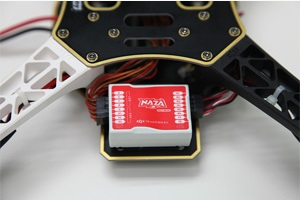
\includegraphics[width = 0.6\textwidth]{Bilder/NAZA_M-lite}
      \par\end{centering}
      \caption[Flightcontroller DJI NAZA-M lite]{Flightcontroller DJI NAZA-M lite\cite{NAZA_M-lite}}
      \label{NAZA_M-lite}
    \end{figure}

    \subsubsection{WLAN}
    Das WLAN-Modul RN171 von welches von Microchip verkauft wird bietet die Schnittstelle zwsichen Server und Hexcaopter. Die Daten können entweder vom Server gesendet
    und vom PIC empfangen werden oder umgekehrt.
    Das WLAM-Modul wird mit einer UART-Schnittstelle betrieben. Für eine Kommunikation sind also nur 2 Leitungen notwendig.
    Es bietet die Möglichkeit über eine Anwendung wie TeraTerm oder HTerm eingestellt zu werden, zusätzlich wird aber auch ein Webinterface angeboten, dieses muss jedoch zuvor
    aktiviert werden.

    \begin{figure}[tbh]
      \begin{centering}
        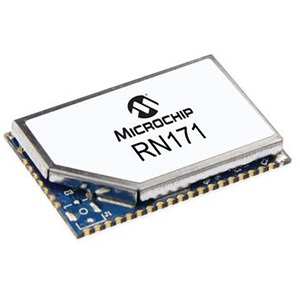
\includegraphics[width = 0.5\textwidth]{Bilder/RN171}
      \par\end{centering}
      \caption[WLAN-Modul RN171]{WLAN-Modul RN171\cite{RN171}}
      \label{RN171}
    \end{figure}

    Die Datenübertragung findet dabei für den Nutzer sehr unproblematisch dar. Einerseits sind konfigurierbare Pins vorhanden um die Verbindung zu steuern und zu überwachen,
    andererseits braucht man sich nicht mehr um das Verpacken der Datenpakete kümmern.

%%%%%%%%%%%%%%%%%%%%%%%%%%%%%%%%%%%%%%%%%%%%%%%%%%%%%%%%%%%%%%%%%%%%%%%%%%%%%%%
\section{Blockschaltbild}
Die einzelnen Komponenten werden über den Mikrocontroller vereint. Sämtliche Berechnungen und Auswertung finden auf diesem statt und werden über diesen ausgegeben \bzw
weitergeleitet. Der Flighcontroller NAZA-M lite wird an die A, E, R und T Pins angeschlossen.
\begin{figure}[H]
  \begin{centering}
    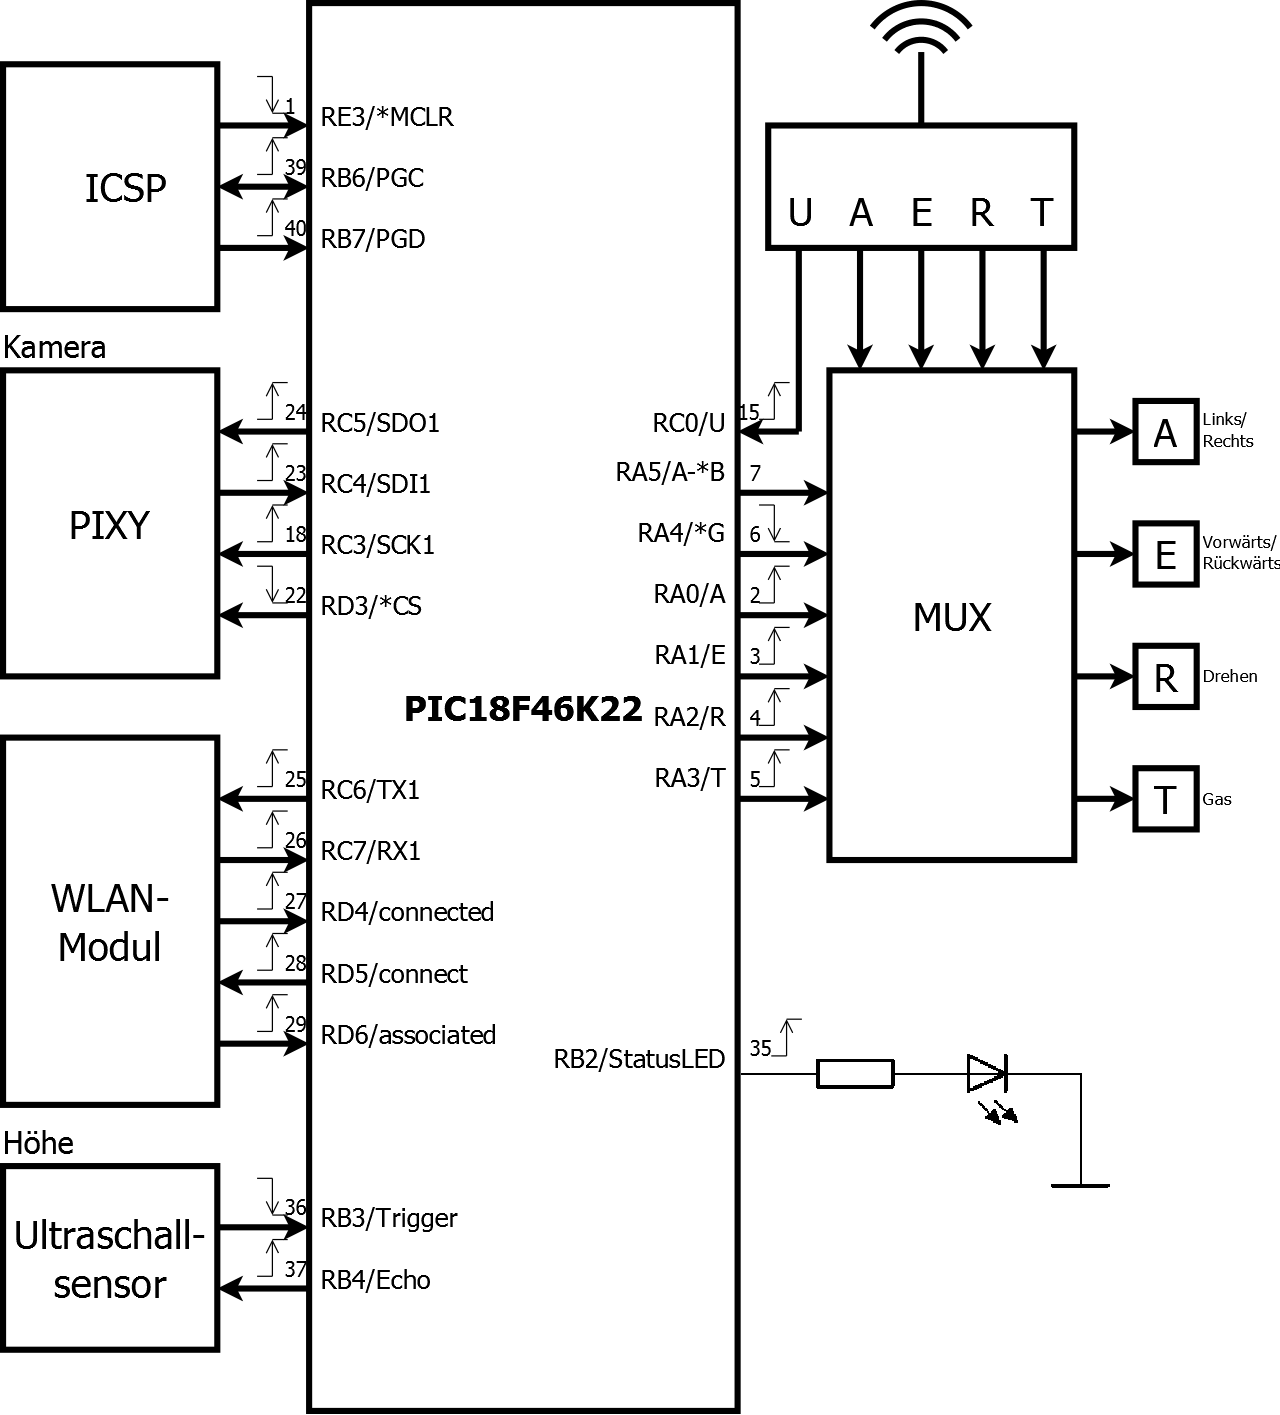
\includegraphics[width = 1\textwidth]{Bilder/Blockschaltbild}
  \par\end{centering}
  \caption{Blockschaltbild der Hauptplatine}
  \label{Blockschaltbild}
\end{figure}
  \subsection{Hauptplatine}

    \subsubsection{Technische Planung}

    \subsubsection{Umsetzung}

    \subsubsection{Herausforderungen und Lösungen}

  \subsection{WLAN}

    \subsubsection{Technische Planung}

    \subsubsection{Umsetzung}

    \subsubsection{Herausforderungen und Lösungen}
